\chapter{Periodic table and energy}
	The focus of this module is inorganic and physical chemistry, the applications of energy use to everyday life and industrial processes, and current environmental concerns associated with sustainability. 

\section{The Periodic table 3.1.1}
	
	\paragraph{Simply put} the periodic table lists the known elements in order of atomic number\footnote{A number derived from the number of protons} and also grouped by periods, or rows, which show the trends in physical and chemical properties.
	
	Groups, or columns, generally contain chemicals of similar properties.
	This is because they all have the same amount of electrons missing in the outer shell\footnote{Sort of true for first three periods}.
	
	\paragraph{First ionisation energy} is the amount of energy required to remove one electron from each atom in one mole of gaseous substance.
	There are several things which affect first ionisation energy which I will now go into.
	The first ionisation energy generally increases as we go across the period and decreases as we go down the group in general. 
	
	This is because as we move across the period the nuclear charge gets greater.
	This then affects the atomic radius, making it smaller.
	This means that the electrons on the outer shells are more attracted to the nucleus and so the first ionisation energy increase.
	
	Take period 2.
	as we go across it and look at the first ionisation energies we see this Li$<$Be$>$B$<$C$<$N$>$O$<$F$<$Ne.
	The question is why is Be$>$B and N$>$O? This doesn't fit with our previous generalisations.
	
	\paragraph{Oddities in the first ionisation energy} The first oddity we see is between Be$>$B.
	This is caused as a result of Be having a full s sub-shell and B having only one electron in the p sub-shell.
	Although a little odd at first glance this should become obvious.
	A full sub-shell is going to need more energy to remove an electron than a sub-shell with only one electron.
	So we see this s-p sub orbital trend in first ionisation energies
	
	The second oddity is the N$>$O. This is caused by p-orbital reputation.
	As the p orbital fills to 4 it looks like this,
	\begin{center}
		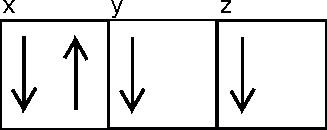
\includegraphics{P4orbital}
	\end{center}
	As we can see the P$_x$ only has gained an electron of opposite spin.
	This causes repulsion which means that this new electron requires less energy to be removed than if we have P$^3$ like in Nitrogen.
	This is called p-orbital repulsion.
	
	\paragraph{Successive ionisation energies} is what we see when we take several electrons away from an element.
	This can be used to predict the number of electrons in each shell.
	Between shells there is a large difference in ionisation energies.
	
	Trends such as these give support to the Bohr model of the atom\footnote{The Bohr model is the model you have been learning}.
	They support the idea that we have a variety of shells with sub-shells.
	
\section{Periodic trend in structure 3.1.1}
	
	\paragraph{Metallic bonding} is the a ``strong electrostatic attraction between cations (positive ions) and delocalised electrons".
	This bonding is between metals as forms giant metallic lattices.
	Metals are able to conduct electricity because of the sea of delocalised electrons created by the metallic bond.
	Metals are almost always solid at room temperature, except for mercury.
	This is because metallic bonding is very strong, but dependent on how many electrons the elements loose as well as well as other factors.
	
	\paragraph{Giant covalent lattices} are, unlike simple molecular lattices, atoms not molecules bonded by covalent bonds.
	This can make for some incredibly strong elements.
	Carbon, boron and silicon are examples of atoms that can form giant covalent lattices.
	Carbon can form Diamond, graphite and graphene.
	
	Other than graphite and graphene, giant covalent lattices will not conduct electricity.
	This is because the electrons are immobile. However graphite has a free electron per carbon atom. 
	These electrons join a sea of delocalised electrons and can move between the layers in the carbon.
	These mobile charge carriers are what allow graphite and graphene to be conductive.
	
	\paragraph{Solubility} Both metals and giant covalent lattices are, on the whole insoluble.
	In the case of metals, they may well react when in polar solvents not dissolve.
	In the case of giant covalent lattices, the bonding is far too strong to be broken by solvents.
	
	\paragraph{Graphene} is the latest wonder chemical.
	It consists of a single layer of graphite, composed of hexagonally linked carbon atoms.
	It has the same electrical conductivity of copper and is the thinnest, strongest element ever made.
	The reason for its electrical conductivity is that it has, like graphite, delocalised electrons.
	Theses act as mobile charge carriers.
	
	There is potential for this to be used in micro-computing to replace silicone, this could server to further decrease the size and cost of computer processors.
	
	\paragraph{Melting points} for giant metallic/covalent structures are very heigh.
	This means the following (for periods 2 and 3):
	\begin{itemize}
		\item As we move from groups 1 to 14 we see a rise in melting temperatures as these elements form \textit{giant structures}.
		\item A sharp drop is seen at group 14 to 15. This is because group 15-18 elements don't form giant structures.
		\item Group 15 to 18 are comparatively low. This is because are \textit{simple molecular structures}.
	\end{itemize}
\section{Group 2 3.1.2}

	\paragraph{s sub-shell} Is filled in all the group two elements.
	This means that they contain two more electrons than the Nobel gas before it.
	In redox reactions these substances loose two electrons and from 2+ ions.
	
	The next part is just revisiting redox and so I will just summarise.
	You should know how group two elements from Mg$\rightarrow$Ba react with water, oxygen and week acids.
	Just know that group 2 elements are oxidised by +2.
	
	\paragraph{Reactivity} increases as we go down the group because the group two elements in a reaction loose electrons.
	So as we learnt before, as we move down the group the first (and in this case second) ionisation energies increase due to greater shielding\footnote{Shielding is where electrons from other shells block, in a sense, the positive attraction on the outer electrons.} and atomic radius (so overall less attraction to the outer s electrons.).
	
\section{The halogens 3.1.3}
	
	\paragraph{Boiling trends} in halogens are caused because of there existence as diatomic molecules.
	The boiling point increases down the group because of the stronger London forces (caused by more electrons).
	
	\paragraph{Redox again} is found here.
	Much the same as all the others but this time they are oxidised.
	This is because they need only gain one electron to have the electron configuration of a noble gas.
	They form anions.
	
	\paragraph{Displacement reactions} occur when a significantly more reactive chemical is reacted with a compound containing a similar, but less reactive, compound.
	Using displacement reactions we can see that reactivity decreases down the group.
	
	\paragraph{Halogen-halide displacement} The reactions are as follows,
	\begin{itemize}
		\item a chloride solution will not be displaced by bromine or iodine. This is because chlorine is the most reactive.
		\item a bromide solution will react when chlorine is added. It will turn orange as the Br$^-$ ions are displaced and so from Br$_2$,
		
			\ch{Cl2(aq) + 2 Br^-(aq) -> 2 Cl^-(aq) + Br2(aq)}
			However given that iodine is less reactive still there will be no reaction between \ch{I2} and bromide.
		\item As the least reactive iodide solution will be displaced by both chlorine and bromine to form a brown solution,
		
			\ch{Cl2(aq) + 2 I^-(aq) -> 2 Cl^-(aq) + I2(aq)}
			
			\ch{Br2(aq) + 2 I^-(aq) -> 2 Br^-(aq) + I2(aq)}
	\end{itemize}
	To tell apart the similar brown and orange we can add a non-polar solvent like cyclohexane to dissolve the halogen.
	When \ch{I2} is dissolved we can see the cyclohexane layer go a deep violet.
	
	\paragraph{The reason for decreasing reactivity} is that it is the opposite to group two.
	To gain an electron we need more attraction.
	As such more shielding and a grater atomic radius just cause less attraction to the electron and make it less reactive.
	
	\paragraph{Disproportionation} is what we call a reaction when the same element undergoes reduction and oxidation.
	This is illustrated by the following,
	\begin{itemize}
		\item The treatment of water with chlorine
		
		\ch{"\ox{0, Cl}" {}2(aq) + H2O(l) -> H "\ox{+1,Cl}" {}O(aq) + H "\ox{-1, Cl}" {}(aq)}
		
		As we can see, Chlorine has been both oxidised and reduced.
		
		\item The reaction of chlorine with cold, dilute aqueous sodium hydroxide,
		
		\ch{"\ox{0, Cl}" {}2(aq) + 2 NaOH(aq) -> Na "\ox{+1, Cl}" {}O(aq) + Na "\ox{-1, Cl}" {}(aq) + H2O(l)}
	\end{itemize}
	
	\paragraph{Water treatment} using chlorine is extremely useful.
	This is because chlorine kills bacteria.
	However, there are some hazards in using chlorine.
	Toxic chlorine gas and the risk of forming carcinogenic chlorinated hydrocarbons (when reacting with plant matter).
	
	\paragraph{The Halide tests} are reactions used to test for halide ions in aqueous solution.
	This is done by adding aqueous silver ions (by using \ch{AgNO3}).
	The ionic equation is as follows (where X is any halide ion),
	
	\begin{center}
		\ch{Ag^+(aq) + X^-(aq) -> AgX(s)}
	\end{center}
	
	As we can see, this reaction creates a precipitate.
	Now we can derive the precise halide ion by looking at the colour of the precipitate.
	Chlorine will form a white precipitate, Bromine a cream and iodine yellow.
	
	Adding dilute aqueous ammonia will dissolve the precipitate AgCl, and by adding concentrated aqueous ammonia we dissolve both AgCl and AgBr.
	
\section{More tests 3.1.4}

	\paragraph{Three tests} you need to know for this section. They need to be done in the following order,
	\begin{enumerate}
		\item Carbonate (\ch{CO3^{2-}(aq)}) test
		\item Sulfate (\ch{SO4^{2-}(aq)}) test
		\item halide (\ch{Cl^-(aq)},\ch{Br^-(aq)} and \ch{I^-(aq)}) test
	\end{enumerate}
	
	\paragraph{Carbonate ions} are tested by adding a dilute acid. It is by the following ionic equations,
	\begin{center}
		\ch{CO3^{2-}(aq) + 2 H^+(aq) -> H2O(l) + CO2(g)}
	\end{center}
	As you can see \ch{CO2} is formed, which is gaseous. So if a \ch{CO3^-(aq)} ion is present we will see effervescence when we add it.
	We will see why we need to do this first.
	(remember to use an acid which will not interfere in the other two tests like \ch{NHO3}.
	
	\paragraph{Sulphate ions} are tested for by adding \ch{Ba^{2+}(aq)}. This is now by the following equations,
	\begin{center}
		\ch{Ba^{2+}(aq) + SO4^{2-} -> BaSO4(s)}
	\end{center}
	We see a white precipitate form (\ch{BaSO4(s)}).
	However this needs to be done after the carbonate test because \ch{Ba^{2+}} ions will form \ch{BaCO3(s)}, which is also a white precipitate.
	
	\paragraph{The halide tests} are mentioned above.
	
	\paragraph{Testing for ammonium ions} is simple. Just react with warm aqueous NaOH,
	\begin{center}
		\ch{OH^-(aq) + NH4^+(aq) -> NH3(g) + H2O(l)}
	\end{center}
	So by adding NaOH we will see the solution effervesce if the NH$_4^+$ ions.
	
\section{Enthalpy 3.2.1}
[For now I am skipping this section due to is easiness. Just apply basic logic and maths]

\section{Rates of Reaction 3.2.2}
	\paragraph{Collision} theory hasn't changed at all from GCSE.
	Sill we look at the microscopic consequences of pressure, concentration and temperature (kinetic energy) on individual molecules.
	Successful collisions are needed which is when the reactive atoms in a molecule collide.
	
	\paragraph{Catalysts} are substances that, when added to a chemical reaction, serve to increase the rate of reaction without reacting itself.
	
	This effect is achieved by the catalyst decreasing the required activation energy, thus providing a faster pathway for the reaction to take place.
	
	\paragraph{Homogeneous catalysts} refers to a catalyst that is in the same state as the reactants.
	This works by forming intermediate products.
	
	\paragraph{Heterogeneous catalysts} are catalysts which differ in state from the reactants.
	These act by a series of absorption and desorption.
	
	\paragraph{Catalysts} have massive importance in industry.
	They are used to reduce the amount of energy (in heat and pressure) in industrial reactions.
	This then reduces the amount of fossil fuels needing to be burnt, thus reducing \ch{CO2}.
	
	\paragraph{Measuring} rates of reaction can be done in many ways. This can involve measuring gas or mass over time.
	
	\paragraph{The Boltzmann distribution} is a frequency distribution used to predict the energy of molecules.
	The area under the curve represents the number of molecules with a given energy.
	The curve changes when the temperature rises (skews negativity). E$_a$ moves to the left when a catalyst is added.
	
\section{Chemical equilibrium 3.2.3}

	\paragraph{A dynamic equilibrium} exists in a closed system when the rate of the forward reaction is equal to the rate of the reverse reaction and the concentrations of reactants and products do not change.
	
	\paragraph{le Chatelier’s principle} states that ``When any system at equilibrium is subjected to change in concentration, temperature, volume, or pressure, then the system readjusts itself to (partially) counteract the effect of the applied change and a new equilibrium is established."
	
	Remember that catalysts do not affect the position of equilibrium as they only affect the activation energy, and the reaction goes both ways so this cancels out.
	
	\paragraph{Investigating equilibrium with concentration} is done by the following,
	
	\begin{center}
		\ch{2 CrO4^{2-}(aq) + 2 H^+(aq) <=> Cr2O7^{2-}(aq) + H2O(l)}
	\end{center}
	This reaction is sensitive to the acid concentration. Adding acid concentration will shift the point of equilibrium to the 'right'.
	We can see this because \ch{CrO4^{2-}(aq)} solution is yellow and \ch{Cr2O7^{2-}(aq)} solution is yellow.
	So by raising the concentration of the acid we see the solution got from yellow to orange.
	Procedure is as follows:
	\begin{enumerate}
		\item Add a solution of yellow potassium chromate to a beaker
		\item Add dilute sulfuric acid drop by drop until there is no further change in colour (orange).
		\item Add aqueous sodium hydroxide until there is no further change in colour (yellow).
	\end{enumerate}
	You have now witnessed equilibrium in action.
	\paragraph{Investigating equilibrium with temperature} is done by the following,
	
	\begin{center}
		\ch{[Co(H2O)6]^{2+}(aq) + 4 Cl^-(aq) <=> CoCl4^{2-}(aq) + 6 H2O(l)}
	\end{center}
	As temperature increases the reaction shifts right (in the endothermic direction) and vice-versa. This reaction can be done by the following steps,
	
	\begin{enumerate}
		\item Dissolve cobalt chloride in a boiling tube. Add a small quantity of hydrochloric acid. Then put the solution in ice to cool it until it turns pink (because \ch{[Co(H2O)6]^{2+}(aq)} solution is pink).
		\item Set up a boiling water bath and transfer the boiling tube. Wait until it turns blue (because \ch{CoCL4^{2-}} is blue).
		\item Transfer back to ice water and observe the change back to pink.
	\end{enumerate}
	And you have now witnessed a shift in equilibrium.
	
\section{The equilibrium constant, $K_c$ 3.2.3}

	\paragraph{Equilibrium constant} is calculated by,
	\begin{center}
		In the reaction $a$A + $b$B \ch{<=>} $c$C + $d$D
		\begin{equation}
			K_c = \frac{[\textnormal{C}]^c[\textnormal{D}]^d}{[\textnormal{A}]^a[\textnormal{B}]^b}
		\end{equation}
	\end{center}
	This requires a little explaining, The A, B, C and D values are the \textit{equilibrium} concentrations of the reactants (in mol dm$^{-3}$).
	
	Where $K_c = 1$ it indicates that the reaction is halfway between reactants and products.
	
	Where $K_c > 1$ it indicates that the position of equilibrium is shifted to the right (the products).
	
	Where $K_c < 1$ it indicates that the position of equilibrium is shifted to the left (the reactants).
	